% --------------------------------------
% Document Class
% --------------------------------------
\documentclass[a4paper,11pt]{article}
% --------------------------------------



% --------------------------------------
% Use Package
% --------------------------------------


\usepackage[francais]{babel}
\usepackage{ucs}
\usepackage[utf8]{inputenc}
\usepackage[T1]{fontenc}

\usepackage{makeidx}
\usepackage{color}
\usepackage{graphicx}
\usepackage{float}
\usepackage[hidelinks]{hyperref} 
\usepackage{geometry}
%\usepackage{lastpage}
%\usepackage{marginnote}
\usepackage{fancyhdr}
%\usepackage{titlesec}
%\usepackage{framed}
\usepackage{amsmath}
\usepackage{empheq}
\usepackage{array}
\usepackage{multicol}
\usepackage{csquotes}
%\usepackage{adjustbox}

% insert code
\usepackage{listings}

% define our color
\usepackage{xcolor}

% code color
\definecolor{ligthyellow}{RGB}{250,247,220}
\definecolor{darkblue}{RGB}{5,10,85}
\definecolor{ligthblue}{RGB}{1,147,128}
\definecolor{darkgreen}{RGB}{8,120,51}
\definecolor{darkred}{RGB}{160,0,0}

% other color
\definecolor{ivi}{RGB}{141,107,185}

\def\verticaltext#1{\rotatebox[origin=c]{90}{\x{#1}}}


\lstset{
    language=python,
    captionpos=b,
    extendedchars=true,
    frame=lines,
    numbers=left,
    numberstyle=\tiny,
    numbersep=5pt,
    keepspaces=true,
    breaklines=true,
    showspaces=false,
    showstringspaces=false,
    breakatwhitespace=false,
    stepnumber=1,
    showtabs=false,
    tabsize=3,
    basicstyle=\small\ttfamily,
    backgroundcolor=\color{ligthyellow},
    keywordstyle=\color{ligthblue},
    morekeywords={include, printf, uchar},
    identifierstyle=\color{darkblue},
    commentstyle=\color{darkgreen},
    stringstyle=\color{darkred},
}


% --------------------------------------



% --------------------------------------
% Page setting
% --------------------------------------
%\pagestyle{empty}
\setlength{\headheight}{15pt}

\setcounter{secnumdepth}{3}
\setcounter{tocdepth}{2}

\makeatletter
\@addtoreset{chapter}{part}
\makeatother 

\hypersetup{       % parametrage des hyperliens
  colorlinks=true,  % colorise les liens
  breaklinks=true,  % permet les retours à la ligne pour les liens 
                    % trop longs
  urlcolor= blue,   % couleur des hyperliens
  linkcolor= black, % couleur des liens internes aux documents 
                    % (index, figures, tableaux, equations,...)
  citecolor= green  % couleur des liens vers les references 
                    % bibliographiques
}

% --------------------------------------

% --------------------------------------
% Information
% --------------------------------------
\title{
  \noindent\hrulefill \\
  \vspace{10mm}
  \textbf{Compte-rendu VisA} \\
  \vspace{5mm}
  TP: Modification de la luminance et la saturation d'une image couleur.
}

\author{Gaëtan DEFLANDRE}
% --------------------------------------

\definecolor{myColor}{rgb}{0.5, 0.1, 0.75}

% --------------------------------------
% Begin content
% --------------------------------------
\begin{document}

\maketitle
\noindent\hrulefill \\


\section*{Introduction}


\newpage

Dans ce TP, nous travaillons avec les images du test d'Ishihara utilisé 
pour déceler le daltonisme.

\begin{figure}[H]
  \begin{center}
    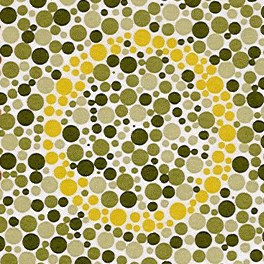
\includegraphics[width=120px]{images/it1_72pp.png}
    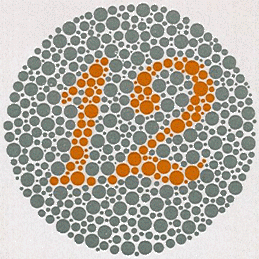
\includegraphics[width=120px]{images/it2_72pp.png}
    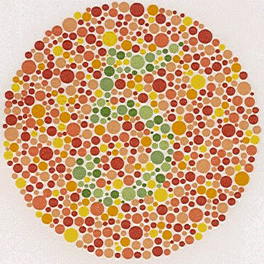
\includegraphics[width=120px]{images/it3_72pp.png}
    \caption{Images originales utiles à ce TP}
  \end{center}
\end{figure}

\section{Manipulation de la luminance}

Dans cet exercice, nous utilisons les images d'origine assombries:

\begin{figure}[H]
  \begin{center}
    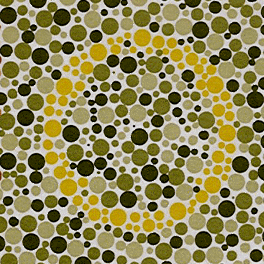
\includegraphics[width=120px]{images/it1_72pp_sombre.png}
    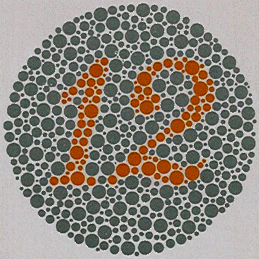
\includegraphics[width=120px]{images/it2_72pp_sombre.png}
    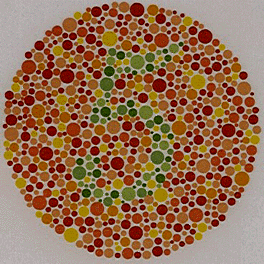
\includegraphics[width=120px]{images/it3_72pp_sombre.png}
    \caption{Images sombres}
  \end{center}
\end{figure}

Pour retrouver, de manière précise, les différences entre l'image 
d'origine et l'image assombrie, il faut choisir le bon espace de
représentation de l'image. Dans notre cas, seule la luminosité 
semble avoir été modifié, ainsi pour trouver aisément cette 
différence, nous choisissons un espace qui contient l'information de 
luminance.\\

Les espaces tels que \textit{Lab} et \textit{Luv} contiennent cette 
information. La valeur \textit{V} de l'espace \textit{HSV} ou le 
\textit{Y} de l'espace \textit{YUV} peuvent être utilisé. Nous 
nous servons de l'espace \textit{Lab} lors de cet exercice.\\

Nous pourrions regarder l'information de chrominance également, 
afin de voir si celle-ci a été modifié.\\

\begin{figure}[H]
  \begin{center}  
    \shortstack{
      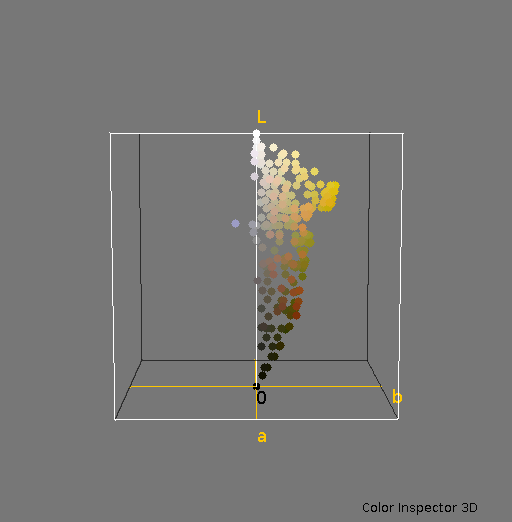
\includegraphics[width=150px]{images/it1.png} \\ 
      \texttt{\small it1\_72pp.bmp}
    }
    \shortstack{
      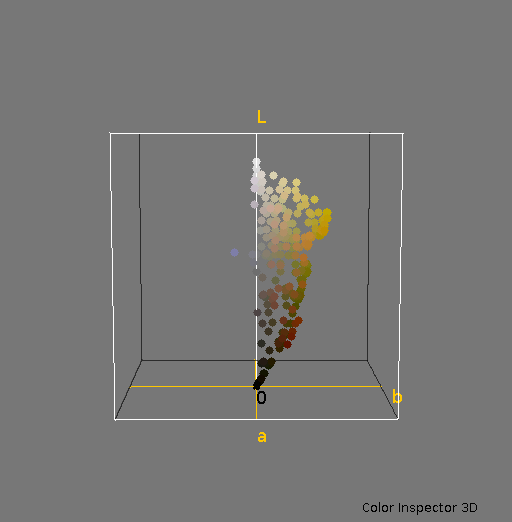
\includegraphics[width=150px]{images/it1_sombre.png}\\
      \texttt{\small it1\_72pp\_sombre.bmp}
    }
    \caption{Diagrammes de it1 originale et assombrie dans l'espace Lab.}
  \end{center}
\end{figure}

Dans l'espace \textit{Lab}, on voit nettement la différence sur l'axe 
de la luminance. La luminance de l'image sombre ne va pas dans les 
tons très clairs, alors que la luminance de l'image d'origine est 
réparti sur tout l'axe \textit{L}.\\

Ainsi, nous pouvons retrouver une valeur $\varphi$ à ajouter à chaque 
canal de \textit{RGB} pour que les images sombres approximent les images
originales.



\begin{table}[H]
  \begin{center}
  
    \begin{tabular}{|l||c|c|c|}
    
      \hline
    
      \bf Images originales &
      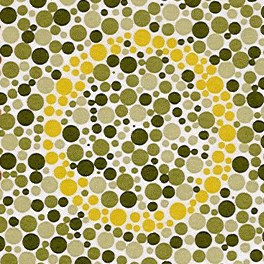
\includegraphics[width=80px]{images/it1_72pp.png} & 
      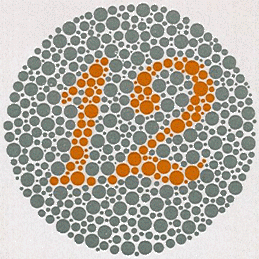
\includegraphics[width=80px]{images/it2_72pp.png} & 
      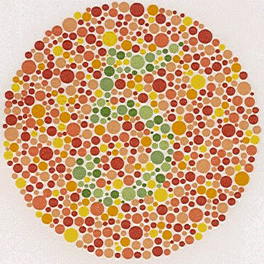
\includegraphics[width=80px]{images/it3_72pp.png} \\
      
      \hline
       
      \bf Images sombres &
      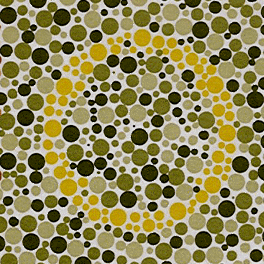
\includegraphics[width=80px]{images/it1_72pp_sombre.png} &
      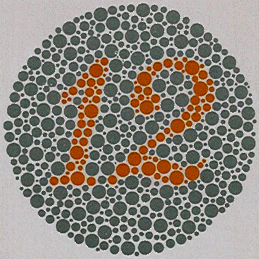
\includegraphics[width=80px]{images/it2_72pp_sombre.png} &
      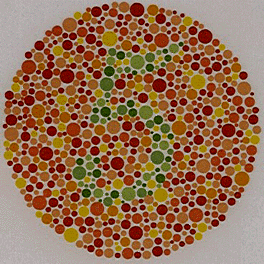
\includegraphics[width=80px]{images/it3_72pp_sombre.png}\\
      
      \hline
      
      \bf Valeur de $\varphi$ &
      30 &
      40 &
      60\\
      
      \hline
    \end{tabular}
    
    \caption{Tableau ajoute de la valeur de $\varphi$ canaux RGB}
    \label{tab:}
    
  \end{center}
\end{table}

Cependant lorsqu'on calcule la différence entre l'image originale et 
l'image résultante après ajout de la valeur $\varphi$. On remarque que 
les images ne sont pas identiques.

\begin{figure}[H]
  \begin{center}  
    \shortstack{
      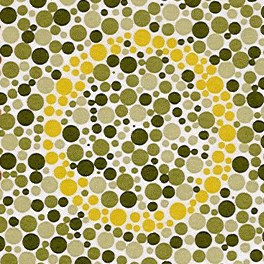
\includegraphics[width=120px]{images/it1_72pp.png} \\ 
      \texttt{\small it1\_72pp.bmp}
    }
    \shortstack{
      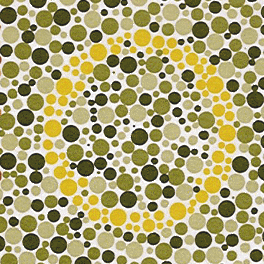
\includegraphics[width=120px]{images/luminance_it1.png}\\
      {\small \texttt{it1\_72pp\_sombre.bmp} + $\varphi$ }
    }\\
    \shortstack{
      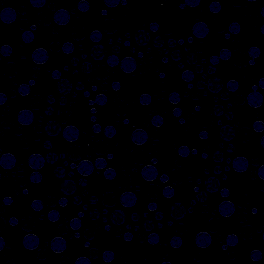
\includegraphics[width=120px]{images/diff_it1.png}\\
      {\small Différence}
    }
    \shortstack{
      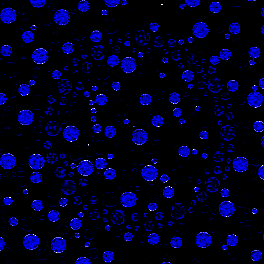
\includegraphics[width=120px]{images/diff_it1_norm.png}\\
      {\small Différence normalisée}
    }
    \caption{La différence non identique}
  \end{center}
\end{figure}

Cette différence est normale comme nous ajoutons la même valeur pour 
chaque canal dans l'espace \textit{RGB}. Or seule la luminance semble
avoir été modifié. De plus, nous distinguons une teinte bleue sur 
l'image de différence. En effet, on ajoute $\varphi$ à la composante 
blue, de l'image sombre, alors que la teinte des pixels de cette image 
est jaune, c'est-à-dire composé de rouge et de vert.\\

Pour régler ce problème, il faut ajouter la valeur $\varphi$ à la 
luminance dans un espace qui la contient. 

\newpage

\section{Rétablissement de la saturation}

Pendant ce second exercice, nous employons les deux images suivantes.

\begin{figure}[H]
  \begin{center}  
    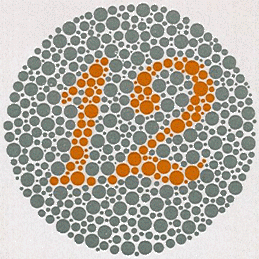
\includegraphics[width=100px]{images/it2_72pp.png}
    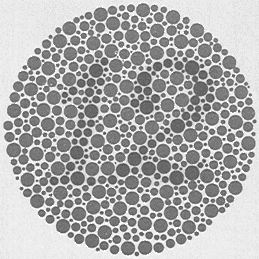
\includegraphics[width=100px]{images/it2_72pp_gris.png}
    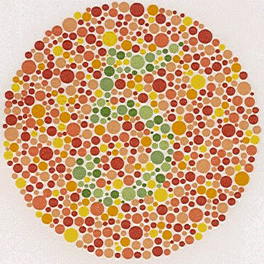
\includegraphics[width=100px]{images/it3_72pp.png}
    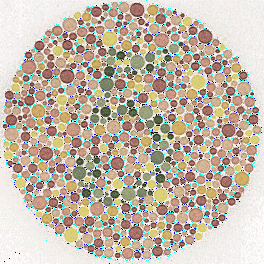
\includegraphics[width=100px]{images/it3_72pp_saturation_faible.png}
    \caption{Images exercice 2}
  \end{center}
\end{figure}

Nous remarquons que l'image grise correspond à l'image \texttt{it2} 
désaturée. Par conséquent, il nous faut un espace colorimétrique qui 
a l'information de chrominance et de saturation. Nous utilisons donc 
l'espace \textit{HSV} qui contient ces informations.

\begin{figure}[H]
  \begin{center}  
    \shortstack{
      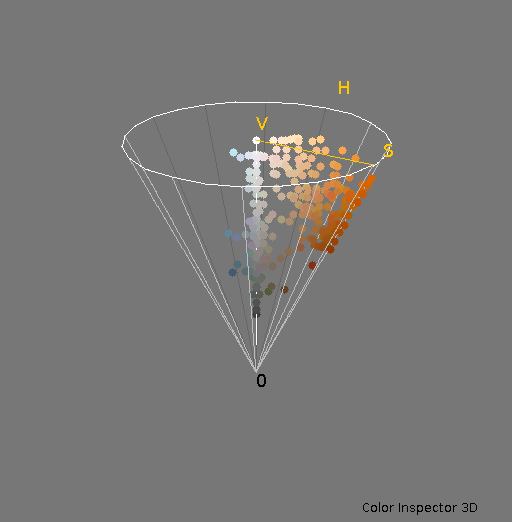
\includegraphics[width=150px]{images/it2.png} \\ 
      \texttt{\small it2\_72pp.bmp}
    }
    \shortstack{
      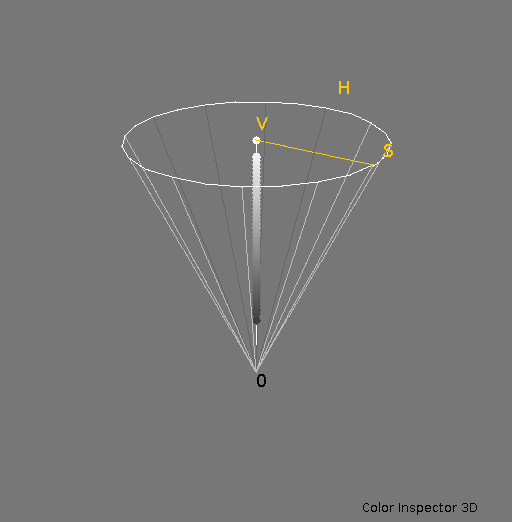
\includegraphics[width=150px]{images/it2_gris.png}\\
      \texttt{\small it2\_72pp\_gris.bmp}
    }

    \caption{Diagrammes de it2 originale et désaturée dans l'espace HSV.}
  \end{center}
\end{figure}

% A partir d'ici l'orthographe n'est pas corrigé

Il est impossible de retrouver l'image \texttt{it2\_72pp} à partir de 
\texttt{it2\_72pp\_gris}, car les informations de saturation et de 
teinte sont perdues. Il faut conserver les informations de saturation 
et de teinte pour retrouver l'image d'origine.\\

Maintenant, nous analysons les images \texttt{it3\_72pp} et 
\texttt{it3\_72pp\_saturation\_faible} dont la saturation a été 
réduite. Pour bien visualiser cette réduction, nous utilisons 
l'espace de \textit{HSB} qui contient l'information de saturation.

\begin{figure}[H]
  \begin{center}  
    \shortstack{
      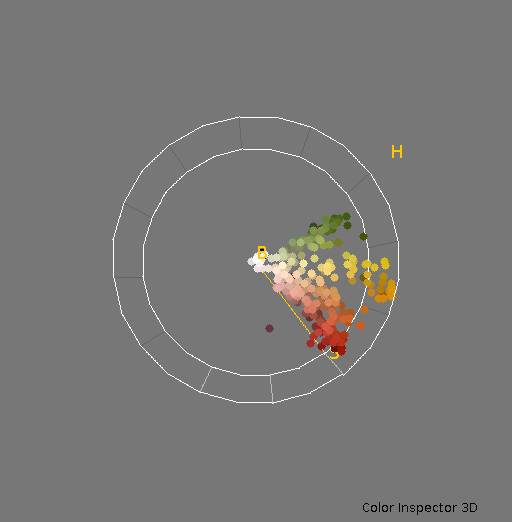
\includegraphics[width=150px]{images/it3.png} \\ 
      \texttt{\small it3\_72pp.bmp}
    }
    \shortstack{
      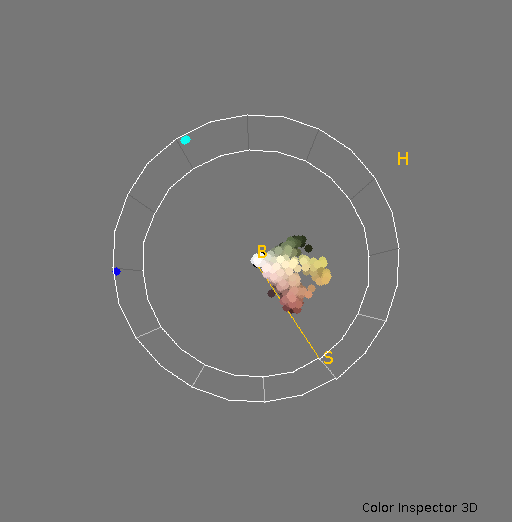
\includegraphics[width=150px]{images/it3_saturation_faible.png}\\
      \texttt{\small it3\_72pp\_saturation\_faible.bmp}
    }
    \caption{Diagrammes de it3 originale et saturation faible dans l'espace HSB.}
  \end{center}
\end{figure}

Approximativement, nous constatons que la saturation a été diviser par 
2.

\begin{table}[H]
  \begin{center}
  
    \begin{tabular}{|c|c|c|}
    
      \hline
    
      \bf Valeur de multication &
      \bf Image résultante &
      \bf Différence \\
      
      \hline
      \hline
      
      1.8 & 
      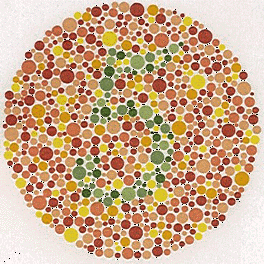
\includegraphics[width=100px]{images/it3_result_1-8.png} &
      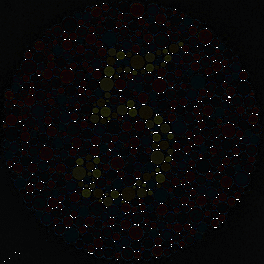
\includegraphics[width=100px]{images/it3_diff_1-8.png}  \\
      
      \hline
      
      2 &
      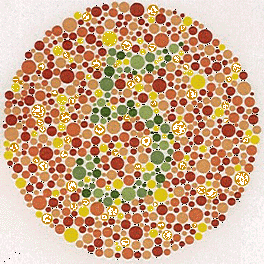
\includegraphics[width=100px]{images/it3_result_2.png} &
      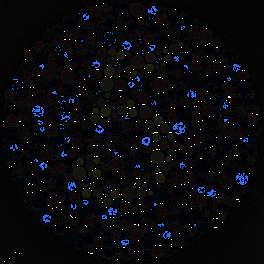
\includegraphics[width=100px]{images/it3_diff_2.png}  \\
      
      \hline
    \end{tabular}
    
    \caption{Tableau de multiplication du canal de saturation}
    \label{tab:}
    
  \end{center}
\end{table}

Nous observons quelques différences car lorsque nous multiplions les 
valeurs de saturation par 2, les valeurs déjà hautes dépassent les 255.

\section{Transformation de la teinte}

Dans cet exercice, nous continuons le travail sur l'image \texttt{it3}. 
En utilisant l"espace \textit{HSB}, nous souhaitons changer la couleur 
du 5, actuellement vert, en bleu. Pour obtenir ce résultat, il suffit 
d'ajouter une valeur au canal de teinte \textit{H} de \textit{HSB}. 
Rappelant que la mesure de la teinte s'effectue entre une valeur de 
0$^{\circ}$ et 360$^{\circ}$, voici le disque chromatique représentant la teinte.\\

\begin{figure}[H]
  \begin{center}
    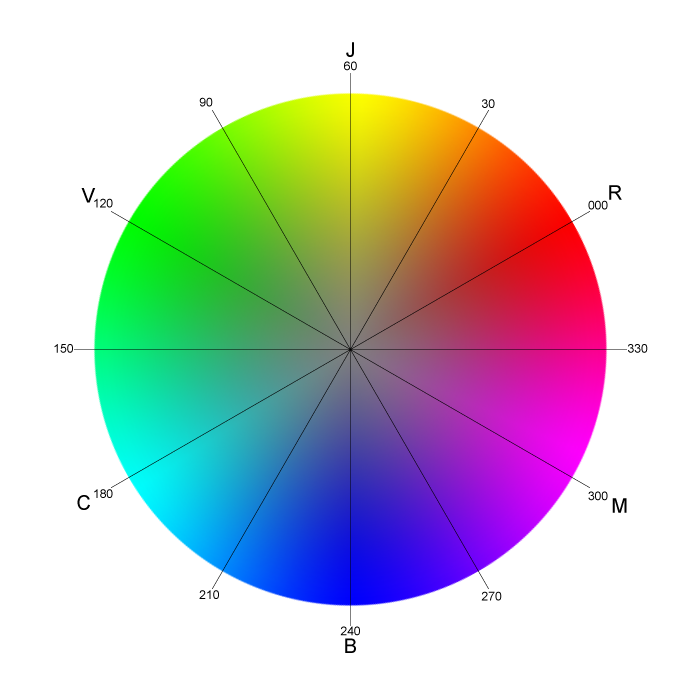
\includegraphics[width=275px]{images/disque_chr.png}
    \caption{Diagramme de teinte}
  \end{center}
\end{figure}

Donc, si nous voulons passer du vert (120$^{\circ}$) au bleu 
(240$^{\circ}$)

\section{Analyse dans des espaces couleur adaptés}

\section*{Conclusion}


\end{document}
